\documentclass{article}
\usepackage[utf8]{inputenc}
\usepackage{amsmath}
\usepackage{upgreek}
\usepackage{amssymb}
\usepackage[]{algorithm2e}
\usepackage{graphicx}
\usepackage{float}

\title{Variational Inference with Coin Toss example}
\author{AntiCodeOn \\ email: {anticodeon@gmail.com}  }
\date{September 2017}


\newcommand\JointProb{p(X,Z,\Theta,\pi,a,b)}
\newcommand\Factorized{q(Z,\Theta,\pi,a,b)}
\newcommand\ProbZGivenpi{\mbox{P(Z)}}
\newcommand\ProbSingleCoin{\Theta_k^{x_n^j}(1-\Theta_k)^{1-x_n^j}}
\newcommand\ProbAllCoins{\Theta_k^{n_H}(1-\Theta_k)^{n_T}}



\newcommand\ProdK{\prod_{k=1}^{K}}
\newcommand\ProdN{\prod_{n=1}^{N}}
\newcommand\ProdJ{\prod_{j=1}^{J}}
\newcommand\SumK{\sum_{k=1}^{K}}
\newcommand\SumN{\sum_{n=1}^{N}}
\newcommand\SumJ{\sum_{j=1}^{J}}

\newcommand\Qfactor{\ProdK{q_k(z_k)}}

\DeclareMathOperator*{\argminA}{arg\,min}

\begin{document}

\maketitle

\section{Introduction}
Variational inference (VI) is a machine learning method for approximation of the difficult to compute probability densities that appear in Bayesian methods. In general, the goal is to find a surrogate distribution over hidden variables and parameters of the original Bayesian model that is close to the original distribution but where the evaluation is computationally efficient. The closeness is defined in terms of a divergence measure between the approximate distribution and the original distribution. 

\section{Motivation}
Consider classical Bayesian setup 
\begin{equation}\label{BayesEq}
p(Z|X) = \frac{p(X,Z)}{p(X)}
\end{equation}
where $X=x_{1:n}$ denotes the observed data while $Z=z_{1:k}$ denotes all the hidden variables and parameters of the model. Numerator of the fraction is called joint distribution
\begin{equation}
    p(X,Z) = p(X|Z)\:p(Z)
\end{equation}
and the denominator (often called evidence) is a marginal distribution
\begin{equation}
    p(X)=\int_{Z}p(X,Z)\:dZ
\end{equation}
Computing the posterior probability is often a very hard problem (for example, due to the exponentially large number of hidden states or because required integrations do not have a closed-form analytical solution). This is why we resort to techniques such as approximation, where the objective is to find a joint distribution $q(Z)$ that replaces original posterior $p(Z|X)$ in a way that enables us to find computationally tractable solutions.
\subsection{Variational inference setup}
Variational inference posits a set of densities $\mathcal{Q}$  over the latent variables $Z$. We typically try to minimize the Kullback-Leibler (KL) divergence
\begin{equation}\label{KL_divergence}
    KL(q(Z)\: ||\: p(Z|X)) = E_{q}\left[log\:\frac{q(Z)}{p(Z|X)}\right]
\end{equation}
of the approximate and the original, true joint distribution
\begin{equation}
    q^*(Z) = \argminA_{q(Z)\in\mathcal{Q}}\: KL(q(Z)\: ||\: p(Z|X))
\end{equation}
KL divergence tells us how much information we loose by choosing the approximate distribution instead of true posterior distribution. 
We can expand the right hand side of (\ref{KL_divergence})
\begin{equation}
KL(q(Z)\: ||\: p(Z|X)) = E_q[q(Z)] - E_q[log\:p(Z|X)]
\end{equation}
Using (\ref{BayesEq}) we get
\begin{equation}
KL(q(Z)\: ||\: p(Z|X)) = p(X) - \underbrace{(E_q[log\:p(X,Z)] - E_q[q(Z)])}_\text{ELBO(q)}
\end{equation}

We want to minimize the KL divergence by varying distribution q(Z). $p(X)$ does not depend on $q$ and is always positive (or equal to zero) so we need to maximize the $ELBO(q)$. The only assumption we are making is that $q(Z)$ factorizes in the following way 
\begin{equation}
q(Z)=\Qfactor{}
\end{equation}
which means that we are breaking possible dependencies between hidden variables in our approximation process.
\begin{equation}
    ELBO(q) = \int q(Z)\: log\:{p(X,Z)}\:dZ - \int q(Z)\:log{\:q(Z)}\:dZ
\end{equation}

\section{Variational inference application}
\begin{equation}
    p(Z|\pi) = \ProdN \ProdK \pi_k^{z_{nk}}
\end{equation}
\begin{equation}
    p(\pi) = Dir(\pi|\alpha_0) = C(\alpha_0)\ProdK{}\pi_k^{\alpha_k-1}
\end{equation}
\begin{equation}
    p(X|Z,\Theta)= \ProdN\ProdK\ProdJ[\ProbSingleCoin{}]^{z_{nk}}
\end{equation}
\begin{equation}
    p(\Theta|a,b) = \ProdK\frac{\Theta^{a-1}(1-\Theta)^{b-1}}{Beta(a,b)}
\end{equation}

Joint distribution is given by
\begin{equation}\label{joint_decomp}
    \JointProb{} = p(X|Z,\Theta)p(Z|\pi)p(\pi)p(\Theta|a,b)
\end{equation}
with factors on the right side of the equation as defined above. Only variables $X={x_1,\dots,x_N}$ were observed. In the next step we consider a variational distribution with the following factorization
\begin{equation}\label{factor_decomp1}
q(Z, \pi, \Theta) = q(Z)q(\pi,\Theta).
\end{equation}
We are separating the latent variables and parameters and this is actually the only assumption we are making.
In order to proceed with the factorization, we use the general result given by Bishop[2006].
\begin{equation}
    ln\: q^*(Z)=E_{\pi,\Theta}[ln\:\JointProb] + const
\end{equation}
For the factor of \textbf{Z} we are only interested in those components of the decomposition \ref{joint_decomp} that depend on \textbf{Z}. All other terms are absorbed into the additive normalization constant, giving:
\begin{equation}
    ln\: q^*(Z)=E_{\pi}[ln\:p(Z|\pi)] + E_\Theta[ln\:p(X|Z,\Theta)] + const
\end{equation}
where
\begin{equation}
    E_{\pi}[ln\:p(Z|\pi)]  = \SumN\SumK z_{nk}E_\pi[ln\:\pi_k]
\end{equation}
and
\begin{equation}
    E_\Theta[ln\:p(X|Z,\Theta)] = \SumN\SumK z_{nk}E_\Theta[\SumJ ln\:\ProbSingleCoin]
\end{equation}
Hence
\begin{equation}
    ln\: q^*(Z)=\SumN\SumK z_{nk}\left(E_\pi[ln\:\pi_k] + E_\Theta[ln\:\ProbAllCoins]\right) + const
\end{equation}
where $n_H$ is a number of heads and $n_T$ number of tails in the n-th experiment.
Proceeding similarly for \textbf{$\pi$} and \textbf{$\Theta$} we get the following expression
\begin{equation}
    ln\: q^*(\pi,\Theta)=E_{Z}[ln\:(\pi) + ln\:p(Z|\pi)] + E_Z[ln\:p(X|Z,\Theta) + ln\:p(\Theta)] + const
\end{equation}
Since there are no expressions that depend on both parameters at the same time we may proceed with the factorization of the parameters independently
\begin{equation}\label{factor_decomp2}
    q(\pi,\Theta) = q(\pi)\:q(\Theta)
\end{equation}
where
\begin{equation}
    ln\:q^*(\pi) = ln\:p(\pi) + E_{Z}[ln\:p(Z|\pi)] + const
\end{equation}
\begin{equation}\label{factor_pi_log}
    ln\:q^*(\pi) = \SumK{(\alpha_k-1)\ln\:\pi_k} + \SumK r_k\:ln\:\pi_k+ const
\end{equation}
where $r_{k} = \SumN E[z_{nk}]$
We have already derived the expectations over $Z$ in EM document.
Taking the exponential of equation \ref{factor_pi_log} we get that the 
\begin{equation}
    q(\pi) = Dir(\pi| \upalpha)
\end{equation}
where $\upalpha$ is vector with K components $\upalpha_k = \alpha_k+r_k$

\begin{equation}
    ln\:q^*(\Theta) = ln\:p(\Theta) + E_Z[ln\:p(X|Z,\Theta)] + const
\end{equation}
\begin{equation}
    ln\:q^*(\Theta) = \SumK (ln\:[\Theta_k^{a_k-1}(1-\Theta_k)^{b_k-1}] + \SumN r_{nk}\SumJ \:ln[\Theta_k^{x_n^j}(1-\Theta_k)^{1-x_n^j}]_ + const
\end{equation}
\begin{equation}
    ln\:q^*(\Theta) = \SumK ln\:[\Theta_k^{a_k-1+n_H{r_k}}(1-\Theta_k)^{b_k-1+n_T{r_k}}] + const
\end{equation}
where $n_H$ equals number of the outcomes of $x_n^j = 1$ (number of heads), and $n_T$ number of the outcomes of $x_n^j = 0$ ( number tails).
We see that the factor for $\Theta$ is Beta distributed variable:
\begin{equation}
    q^*(\Theta) = \ProdK Beta(\Theta|A, B)
\end{equation}
where $A$ is a vector with parameter components $a = a_{k}+n_H{r_k}$ and $B$ with components $b = b_{k}+n_T{r_k}$.
\section{Variational lower bound}
Variational lower bound $L$ is given by 
\begin{equation}
    L = E[ln\:\JointProb{}] - E[ln\:\Factorized{}]
\end{equation}
Using results from \ref{joint_decomp}, \ref{factor_decomp1} and \ref{factor_decomp2}
this simplifies to
\begin{equation}
\begin{split}
    L =& E[ln\:p(X|Z,\Theta)] + E[ln\:p(Z|\pi)] + E[ln\:p(\pi)] + E[ln\:p(\Theta|a,b)] \\
    & -E[ln\:q(Z)] - E[ln\:q(\pi)] - E[ln\:q(\Theta)]
\end{split}        
\end{equation}
We write down each of the terms separately:
\begin{equation}
    E[ln\:p(\pi)] = ln\:C(\alpha_0)+\SumK (\alpha_k-1)(\psi(\alpha_k)-\psi(\SumK \alpha_k))
\end{equation}
\begin{equation}
    E[ln\:p(\Theta_k|a,b)]=\SumK -ln\:Beta(a_k,b_k)+(a_k-1)\psi(a_k)-(b_k-1)\psi(b_k)+(a_k+b_k-2)\psi(a_k+b_k)
\end{equation}
\begin{equation}
    E[ln\:p(Z|\pi) = \SumN\SumK r_{nk}(\psi(\alpha_k)-\psi(\SumK \alpha_k))
\end{equation}
\begin{equation}
    E[ln\:p(X|Z,\Theta)] = \SumN\SumK r_{nk}[n_H(\psi(a_k)-\psi(a_k+b_k))+n_T(\psi(b_k)-\psi(a_k+b_k))]
\end{equation}
\section{Algorithm}
\textit{This section should contain algorithmic description of the problem}
\begin{center}

\begin{algorithm}[H]
 \KwData{Data $X_{1:n}$, number of components K}
 \KwResult{Variational densities $q(\Theta_k;a_k,b_k)$ and $q(z_{nk}, \alpha_k$}
 initialization\;
 \While{the ELBO has not converged }{
  read current\;
  \eIf{understand}{
   go to next section\;
   current section becomes this one\;
   }{
   go back to the beginning of current section\;
  }
 }
 \caption{How to write algorithms}
\end{algorithm}
\end{center}
\section{Results}
\begin{figure}[H]
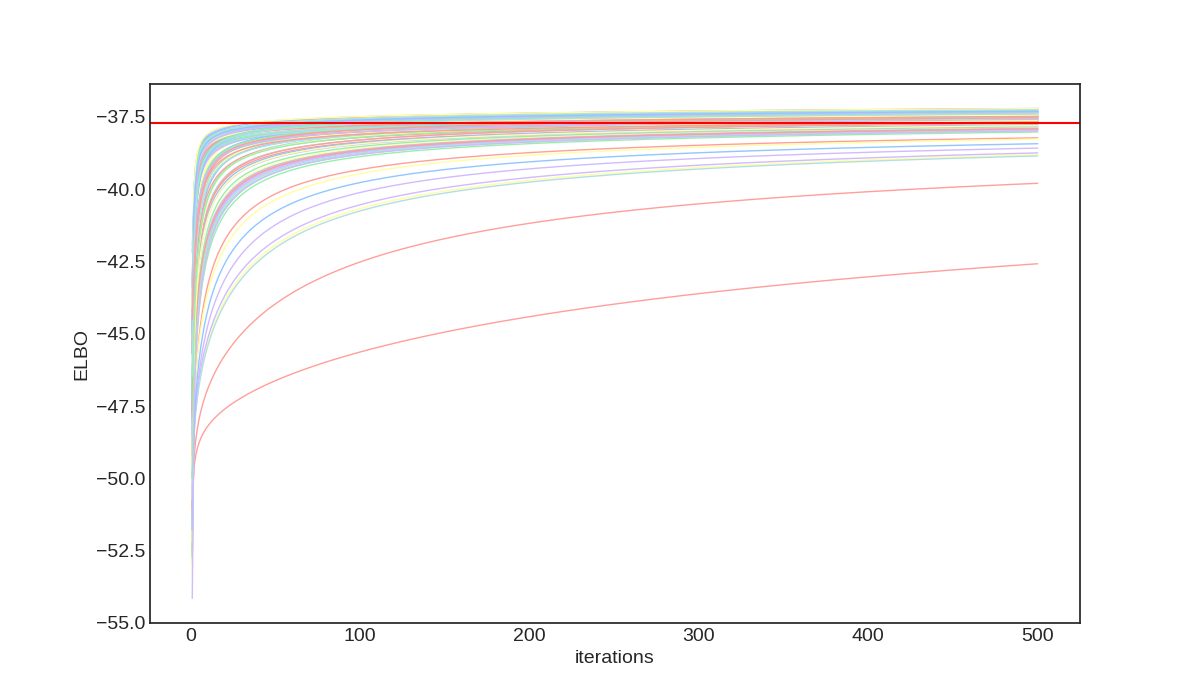
\includegraphics[width=\textwidth]{ELBO_Convergence}\label{elbo:conv}
\caption{Different initialization converge to different local optima of the ELBO}
\end{figure}
\textbf{Initialization.} The ELBO is generally a non-convex objective function. Convergence to the local optimum is guaranteed, however, it can be sensitive with regard to the initialization. Figure \ref{elbo:conv} shows the ELBO convergence for 100 random initializations of the model parameters. Red line denotes the average of the convergence asymptote for all runs. 
\textbf{Convergence.} We define the treshold for the change of ELBO value between subsequent algorithm iterations. Once this difference has fallen under the treshold the procedure stops.
\textbf{Calculation}. During the calculation of the coefficient (which may grow arbitrarily large) we have encountered the problems with the calculation of the normalization coefficient for Dirichlet distribution. Replacing the hand-crafted version with the one from \textit{scipy} package resolved the problem.
\section{Conclusion}
We described variational inference algorithm with mean-field approximation. We have derived parameter update equations for a simple mixture model. Evidence lower bound optimization procedure was used as a criteria for algorithm convergence. We have choosen probability distribution from exponential family 
\end{document}
